\lysh{15009}{2}
\begin{alist}
\item Η συνάρτηση είναι της μορφής $f(x) = \rho \syn  x$, $x \in \mathbb{R}$ με $\rho = -3 < 0$, οπότε η ελάχιστη τιμή της είναι ίση με $-3$ και η μέγιστη τιμή της είναι ίση με $3$.
\item Η συνάρτηση είναι της μορφής $f(x) = \rho \syn (\omega x)$ με $\omega = 1$. Άρα η περίοδος της συνάρτησης $f$ είναι $T = \dfrac{2\pi}{\omega} = \dfrac{2\pi}{1} = 2\pi$.
\item Το σχήμα Α) είναι η γραφική παράσταση της $f(x) = -3\syn  x, x \in \mathbb{R}$, γιατί είναι η μόνη που έχει μέγιστη τιμή $3$ για $x = \pi$ και ελάχιστη $-3$ για $x = 0$ και $x = 2\pi$.
\begin{center}
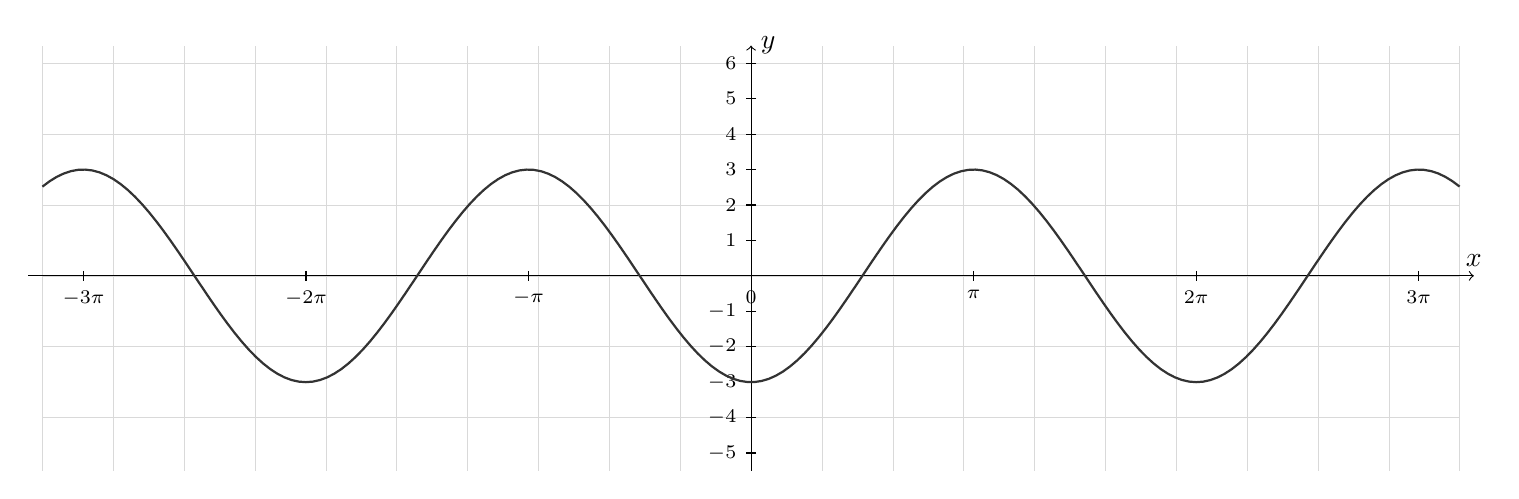
\begin{tikzpicture}[x=1cm,y=0.5cm,scale=0.9]
\draw[step=1cm,gray!30,very thin] (-10,-5.5) grid (10,6.5);
\draw[->] (-10.2,0) -- (10.2,0) node[above] {$x$};
\draw[->] (0,-5.5) -- (0,6.5) node[right] {$y$};
\foreach \x/\xtext in {-9.42/-3\pi, -6.28/-2\pi, -3.14/-\pi, 0/0, 3.14/\pi, 6.28/2\pi, 9.42/3\pi} {
  \draw (\x, 2pt) -- (\x, -2pt) node[anchor=north] {\scriptsize $\xtext$};
}
\foreach \y/\ytext in {-5/-5, -4/-4, -3/-3, -2/-2, -1/-1, 1/1, 2/2, 3/3, 4/4, 5/5, 6/6} {
  \draw (2pt, \y) -- (-2pt, \y) node[anchor=east] {\scriptsize $\ytext$};
}
\draw[black!80, thick, domain=-10:10, samples=200] plot (\x,{-3*cos(\x r)});
\end{tikzpicture}
\end{center}
\end{alist}

